\section{Abnahme}
Die Abnahme erfolgt durch einen abschließenden Vergleich der umgesetzten Funktionen mit den aus der Anforderungsanalyse in Kapitel~4 hervorgegangenen Anforderungen.
Die entwickelte WordClock erfüllt die funktionalen Anforderungen an die kontinuierliche Anzeige der Uhrzeit in Wortform.  
Zusätzlich werden die geforderten Zusatzfunktionen zur Anzeige von Sekunden, Außentemperatur, Wetterzustand, Innenraumtemperatur, Luftfeuchtigkeit, Tageszeit und Mondphase bereitgestellt.  
Die Anzeige der Informationen erfolgt entsprechend der definierten Anforderungen über separate \gls{led}-Strukturen.  
Die Anforderungen an die Hardware werden ebenfalls erfüllt.  
Die Ansteuerung der drei kaskadierten \gls{led}-Stränge arbeitet stabil und zuverlässig.  
Auch die Einbindung des Temperatur- und Feuchtigkeitssensors sowie die stabile Spannungsversorgung des Systems können bestätigt werden.  
Die implementierten Softwarefunktionen erfüllen die definierten Anforderungen an Zeitverarbeitung, Wetterklassifikation und Echtzeitdarstellung.  
Die Synchronisation über \gls{ntp} arbeitet zuverlässig und ermöglicht eine kontinuierlich korrekte Zeitanzeige.  
Ebenso funktioniert die Verarbeitung der Wetterdaten sowie die regelbasierte Umwandlung numerischer Werte in sprachliche Darstellungen fehlerfrei.  
Auch die Anforderungen an die Schnittstellen werden erfüllt.  
Die \gls{wlan}-Anbindung ermöglicht eine stabile Kommunikation mit externen Diensten.  
Zusätzlich arbeitet die \gls{api}-Anbindung zur Wetterdatenabfrage zuverlässig.  
Die bereitgestellte \gls{html}-Benutzeroberfläche ermöglicht die Steuerung von Anzeigeparametern sowie die Darstellung relevanter Betriebsinformationen.  
Die definierten Performance-Anforderungen werden ebenfalls eingehalten.  
Die Anzeige reagiert ohne wahrnehmbare Verzögerungen auf Änderungen der Zeit- und Wetterdaten.  
Auch die Benutzerinteraktion über die Weboberfläche erfolgt ohne auffällige Verzögerungen.  
Die nichtfunktionalen Anforderungen hinsichtlich Zuverlässigkeit, Wartbarkeit und Benutzerfreundlichkeit werden erfüllt.  
Während der Dauerbetriebstests treten keine Fehlfunktionen auf.  
Die modulare Struktur der Software erleichtert zudem die Erweiterbarkeit und Wartung des Systems.  
Weiterhin werden die optischen Anforderungen erfüllt.  
Die Anzeige besitzt eine gleichmäßige Ausleuchtung sowie eine ausreichende Helligkeit zur klaren Erkennbarkeit der dargestellten Wörter.  
Lokale Überhellungen oder störende Blendwirkungen treten nicht auf.  
Zusätzlich wird eine homogene Darstellung erreicht.  

Insgesamt zeigt die Abnahme, dass die entwickelte WordClock die definierten Anforderungen erfüllt und im praktischen Betrieb zuverlässig arbeitet.
Die Abb.~\ref{fig:Montiert} zeigt das Ergebnis dieser Studienarbeit, die entwicklete WordClock an ihrem Installationsort.
\todo{Bild fehlt noch}
\begin{figure}[H]
    \centering
    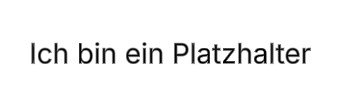
\includegraphics[width=1.0\linewidth]{inhalt/bilder/Platzhalter.jpg}
    \caption[Erfolgreich inbetriebgenommene WordClock]{Die, in dieser Studienarbeit entwickelte, konstruierte, aufgebaute und erfoglreich inbetriebgenommene WordClock, mit funktionalen Zusatzinformationen und Smart-Home-Integration.}
    \label{fig:Montiert}
\end{figure}  